\chapter{関連研究}
\label{related}
%他人の先行研究・事例で、自分の研究が戦う相手について述べて比較する

本章では、本研究の関連研究を示す。

\section{機械学習を用いた利用規約からの未知条項の抽出に関する研究(中村ら 2018)}

\section{CLAUDETTE: an automated detector of potentially unfair clauses in online terms of service(Lippiら 2019)}
CLAUDETTEは、

\section{利用規約中の不公平文の自動検出(青山ら 2019)}

\section{力約: ソフトウェアインストール時における利用規約に応じた力覚提示デバイスの開発(豊島ら 2015)\cite{weko_145305_1}}
力約\cite{weko_145305_1}は、利用規約に同意する際の「同意し契約を交わそうとしている内容の重大さ」に着目し、その重大さをユーザーに伝えるための図\ref{img:rikiyaku}に示すボタン型デバイスを提案している。利用規約を読み飛ばしてしまうという事象を、利用規約の読解の後の同意を押すタイミングでデバイスを利用し、規約内容に応じて「力覚」に作用させることで、より内容の重大さを訴えかけることを試みている。この研究は、同意の重大さを利用者が感じ取ることの困難性を示しており、利用規約の同意ボタンを物理的かつ内容による必要な力の強さの調整を試みている。本研究では、利用規約の重大さについて、ハイライトを持ってより注目を促すように作用をさせている。そのことにより、より条文の内容を読み込むように促せていると考えられる。
\begin{figure}[h]
  \begin{center}
      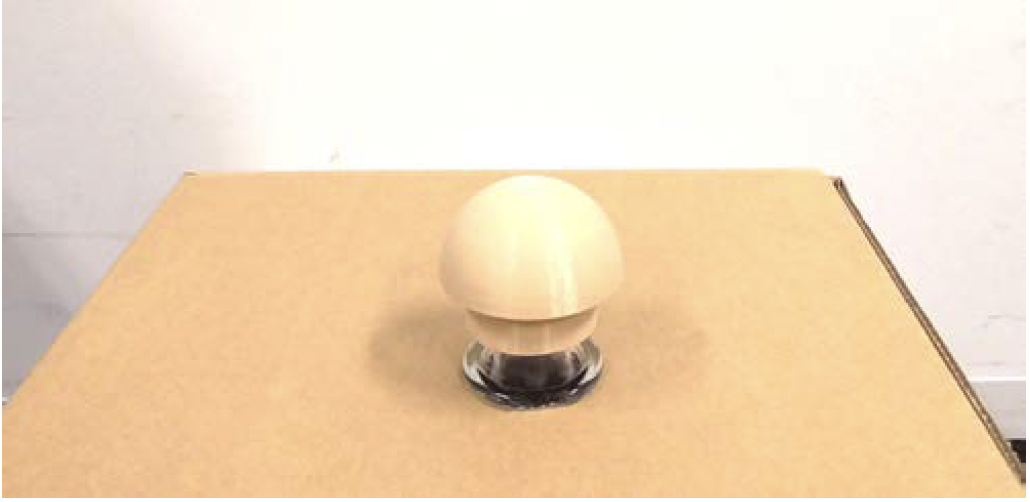
\includegraphics[width=13cm]{img/rikiyaku.png}
      \caption{力約ボタンの外観、文献\cite{weko_145305_1} より引用}
      \label{img:rikiyaku}
  \end{center}
\end{figure}

%%% Local Variables:
%%% mode: japanese-latex
%%% TeX-master: "../thesis"
%%% End:
